% This text is proprietary.
% It's a part of presentation made by myself.
% It may not used commercial.
% The noncommercial use such as private and study is free
% May 2007
% Author: Sascha Frank 
% University Freiburg 
% www.informatik.uni-freiburg.de/~frank/
%
% 
\documentclass[hyperref={pdfencoding=unicode}]{beamer}
\usepackage[latin1]{inputenc}
\usepackage[brazil]{babel}
\usepackage{movie15}
\usepackage{color}




%Temas
\usetheme[compress]{Dresden}
%\useoutertheme[subsection=false]{smoothbars}
%\useinnertheme[shadow]{rounded}
\useinnertheme{rectangles}


\makeatletter
\beamer@theme@subsectionfalse
\makeatother





\begin{document}
\title[Vistas Explodidas]{Vistas Explodidas}
\author[F�bio Markus Miranda - Apresenta��o parcial (INF2062)]{F�bio Markus Nunes Miranda\\fabiom@gmail.com}
\date[\today]{Apresenta��o parcial\\T�picos em Simula��o e Visualiza��o (INF2062)\\Prof. Waldemar Celes\\PUC-Rio}

\begin{frame}
\titlepage
\end{frame}

\begin{frame}
\frametitle{Sum�rio}
\tableofcontents
\end{frame}


\AtBeginSection[\subsection*{}]{\subsection*{}
  \begin{frame}<beamer>%
    \frametitle{Sum�rio: \insertpart}%
    \tableofcontents[currentsection,currentsubsection]%
  \end{frame}%
}% inserts a dummy subsection for the navigation bars






\section{Introdu��o}
Um problema t�pico na visualiza��o de modelos complexos, como motores, pe�as industriais e dispositivos eletr�nicos, � que as caracter�sticas mais interessantes podem estar obstru�das por outras partes menos importantes. T�cnicas de visibilidade inteligente \cite{Viola-05-Smart} levam em considera��o a relev�ncia dos objetos e suas caracter�sticas, e n�o apenas o seu posicionamento no espa�o, permitindo um maior entendimento do objeto em quest�o.

Uma das t�cnicas de visibilidade � a \emph{vista explodida}, desenvolvida ao longo de s�culos na �rea de ilustra��o t�cnica, e agora utilizada para a visualiza��o de modelos 3D. O seu conceito b�sico � modificar o posicionamento de partes de um modelo para facilitar a vis�o de caracter�sticas importantes. Ao contr�rio de t�cnicas como \emph{ghosted view} e \emph{cut away view}, a vista explodida permite a visualiza��o de um modelo sem que se perca qualquer tipo de informa��o sobre ele, j� que n�o h� nenhum tipo de transpar�ncia ou remo��o de partes mais externas. O usu�rio pode ent�o, baseado em sua experi�ncia, reconstruir mentalmente o modelo e assim ter uma vis�o global e o relacionamento entre as partes que o constituem.

\begin{figure}[h]
	\center{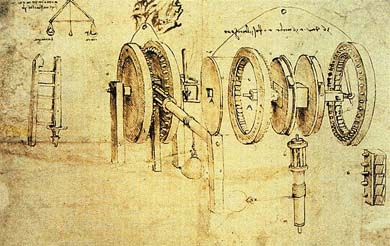
\includegraphics[height=0.5\linewidth]{img/davinci.png}}
	\caption[]{\label{fig:davinci} Exemplo de uma ilustra��o de vista explodida de Leonardo da Vinci.}
\end{figure}

Este trabalho implementa uma t�cnica de vista explodida apresentada em \cite{1360700}. O trabalho busca diminuir a desordem visual ao mesmo tempo que minimiza as dist�ncias de explos�o, facilitando assim o entendimento das rela��es entre as partes do modelo. Para isso, � proposto a constru��o de um \emph{grafo de explos�o}, que ir� ditar a ordem e a dire��o com que cada parte poder� ser explodida. O usu�rio poder� escolher quais partes deseja visualizar e o sistema ir� expandir (ou colapsar) de acordo com o que foi previamente gerado no grafo.

O objeto principal aqui � dar uma vis�o geral sobre o tema, explicar o trabalho escolhido, assim como a sua implementa��o, discutir dificuldades e facilidades e apresentar poss�veis propostas para trabalhos futuros.

Este trabalho est� dividido da seguinte forma: na Se��o \ref{trabalhosrelacionados} s�o apresentados os trabalhos relacionados. A Se��o \ref{metodologia} apresenta uma vis�o geral do sistema de vista explodida, sendo que detalhes de implementa��o s�o discutidos na Se��o \ref{implementacao}. Os resultados s�o mostrados na Se��o \ref{resultados}. A conclus�o e poss�veis trabalhos futuros est�o na Se��o \ref{conclusao}.
\section{T�cnicas de gerenciamento de oclus�o}
\begin{frame}\frametitle{\emph{A Taxonomy of 3D Occlusion Management for Visualization} \cite{1446259}} 
\begin{itemize}
	\item Apresenta uma classifica��o das t�cnicas de gerenciamento de oclus�o, sendo poss�vel perceber de forma objetiva as diferen�as entre as diversas t�cnicas.
	\item A partir de 25 caracter�sticas, o trabalho deriva 5 \emph{patterns} para reduzir a oclus�o em modelos 3D.
\end{itemize}
\end{frame}

\begin{frame}\frametitle{Caracter�sticas das t�cnicas de gerenciamento de oclus�o (1)}
\begin{itemize}
	\item \textbf{Prop�sito principal}:
	\begin{itemize}
		\item \textbf{Descoberta}: tem como objetivo fazer com que o usu�rio fique ciente de partes obstru�das, n�o necessariamente deixando mais acess�vel as informa��es do objeto.
		\item \textbf{Acesso}: diferentemente da \textbf{descoberta}, deixa necessariamente as informa��es do objeto mais acess�veis.
		\item \textbf{Relacionamento espacial}: busca deixar o contexto em que o objeto est� inserido vis�vel e mais f�cil de ser entendido pelo usu�rio. 
	\end{itemize}
\end{itemize}
\end{frame}
	
	
\begin{frame}\frametitle{Caracter�sticas das t�cnicas de gerenciamento de oclus�o (2)}
\begin{itemize}
	\item \textbf{Poder de desambigu��o}
	\begin{itemize}
		\item \textbf{Proximidade}:
		\item \textbf{Interse��o}:
		\item \textbf{"Acercar" (\emph(enclosement))}:
		\item \textbf{Confinamento}:
	\end{itemize}
	\begin{center}
		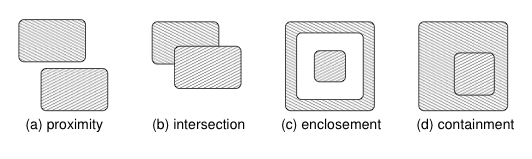
\includegraphics[width=\linewidth]{img/objectInteractions}
	\end{center}
\end{itemize}
\end{frame}
	
\begin{frame}\frametitle{Caracter�sticas das t�cnicas de gerenciamento de oclus�o (3)}
\begin{itemize}
	\item \textbf{Sugest�es de profundidade (\emph{depth cues})}:
	\begin{itemize}
		\item \textbf{Baixa}:
		\item \textbf{Ligeiramente baixa}:
		\item \textbf{M�dia}:
		\item \textbf{Ligeiramente alta}:
		\item \textbf{Alta}:
	\end{itemize}
\end{itemize}
\end{frame}
	
\begin{frame}\frametitle{Caracter�sticas das t�cnicas de gerenciamento de oclus�o (4)}
\begin{itemize}
	\item \textbf{Tipos de vis�o}:
	\begin{itemize}
		\item \textbf{\emph{Single view}}:
		\item \textbf{\emph{Twin separeta views}}:
		\item \textbf{\emph{Twin integrated views}}:
		\item \textbf{\emph{Multiple separate views}}:
		\item \textbf{\emph{Multiple integrated views}}:
	\end{itemize}
\end{itemize}
\end{frame}
	
\begin{frame}\frametitle{Caracter�sticas das t�cnicas de gerenciamento de oclus�o (5)}
\begin{itemize}
	\item \textbf{Modelo de intera��o}:
	\begin{itemize}
		\item \textbf{Passivo}:
		\item \textbf{H�brido}:
		\item \textbf{Ativo}:
	\end{itemize}
\end{itemize}
\end{frame}
	
\begin{frame}\frametitle{Caracter�sticas das t�cnicas de gerenciamento de oclus�o (6)}
\begin{itemize}
	\item \textbf{Invariantes do objeto}:
	\begin{itemize}
		\item \textbf{Posi��o e orienta��o}:
		\item \textbf{Geometria}:
		\item \textbf{Apar�ncia}:
	\end{itemize}
\end{itemize}
\end{frame}



\begin{frame}\frametitle{Classifica��o}
	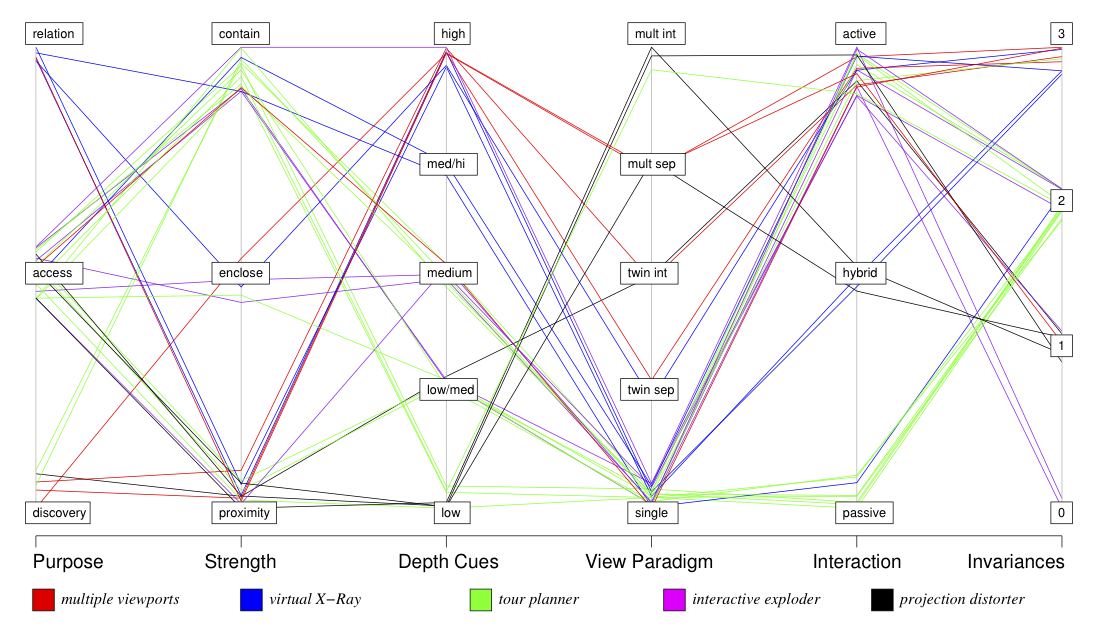
\includegraphics[width=\linewidth]{img/classification}
\end{frame}

\begin{frame}\frametitle{Classifica��o}
	\begin{columns}[T]
	\begin{column}{3cm}
	\begin{itemize}
		\item \alert<1>{Cut-away view, Ghosted View}
		\item \alert<2>{Exploders}
	\end{itemize}
	\vspace{3cm} 
	\end{column}
	\begin{column}{7cm}
	\begin{overprint}
		\includegraphics<1>[height=100.0px]{img/xray}
		\includegraphics<2>[height=100.0px]{img/exploder}
	\end{overprint}
	\end{column}
	\end{columns}
\end{frame}
\section{Trabalhos sobre vistas explodidas}

%\subsection{Illustrative visualization: new technology or useless tautology?}
\begin{frame}\frametitle{\emph{Illustrative visualization: new technology or useless tautology?} \cite{1408633}} 
\begin{itemize}
	\item Visualiza��o ilustrativa: Representa��o visual interativa e expressiva, assistida por computador, motivada por ilustra��es tradicionais. Dois n�veis de abstra��o:
	\begin{itemize}
		\item Abstra��es de baixo n�vel: \textbf{como} renderizar as caracter�sticas de interesse (ex: \emph{toon shading}).
		\item Abstra��es de alto n�vel: \textbf{o que} renderizar. (ex: \emph{cutaways} e vistas explodidas).
				\begin{itemize}
					\item Necessitam de informa��es sobre a relev�ncia dos dados.
					\item \emph{Smart visibility techniques} \cite{Viola-05-Smart}.
				\end{itemize}
	\end{itemize}
\end{itemize}	
\end{frame}


\begin{frame}\frametitle{\emph{Illustrative visualization: new technology or useless tautology?} \cite{1408633}} 
	\begin{columns}
		\begin{column}[c]{5cm}
			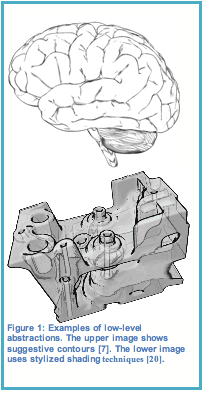
\includegraphics[width=0.6\linewidth]{img/lowlevelabstraction.png}
			\vspace{0cm} 
		\end{column}
		\begin{column}[c]{5cm}
			\begin{overprint}
			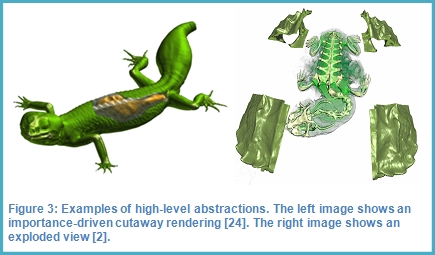
\includegraphics[width=0.8\linewidth]{img/highlevelabstraction.jpg}
			\end{overprint}
		\end{column}
	\end{columns}
\end{frame}



	




				
\subsection{Exploded Views for Volume Data}
\begin{frame}\frametitle{\emph{Exploded Views for Volume Data} \cite{1187828}} 
\begin{itemize}
	\item 
\end{itemize}	
\end{frame}
%\subsection{Smart Visibility in Visualization}
\begin{frame}\frametitle{\emph{Smart Visibility in Visualization} \cite{Viola-05-Smart}} 
\begin{itemize}
	\item 
\end{itemize}	
\end{frame}
\subsection{Designing effective step-by-step assembly instructions}
\begin{frame}\frametitle{\emph{Designing effective step-by-step assembly instructions} \cite{882352}} 
\begin{itemize}
	\item 
\end{itemize}	
\end{frame}
\subsection{Non-invasive interactive visualization of dynamic architectural environments}
\begin{frame}\frametitle{\emph{Non-invasive interactive visualization of dynamic architectural environments} \cite{641493}} 
\begin{itemize}
	\item 
\end{itemize}	
\end{frame}
\subsection{Interactive cutaway illustrations of complex 3D models}
\begin{frame}\frametitle{\emph{Interactive cutaway illustrations of complex 3D models} \cite{2667077}} 
\begin{figure}[ht]
\includemovie[
  inline=false, %nao inclui arquivo no pdf final
  poster,
  text={\small{Carregando v�deo: cutaways-SIG07.mov}}
]{6cm}{6cm}{videos/cutaways-SIG07.mov}
\end{figure}
\end{frame}
\subsection{Automated generation of interactive 3D exploded view diagrams}
\begin{frame}\frametitle{\emph{Automated generation of interactive 3D exploded view diagrams} \cite{1360700}} 
\begin{itemize}
	\item Elabora o trabalho apresentado em \cite{882352}.
	\item Leva em considera��o "grupos" de partes do objeto.
	\item Trata tamb�m casos em que as partes est�o "cercadas".
	\item Maior controle sobre o que � explodido.
\end{itemize}
\begin{center}
	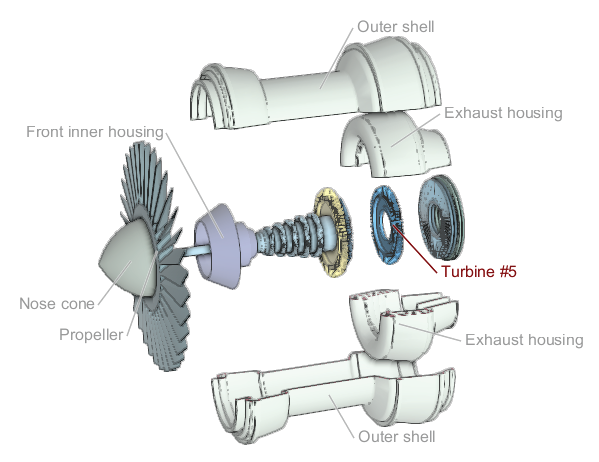
\includegraphics[height=125.0px]{img/exview3D-SIG08_1}
\end{center}
\end{frame}



\begin{frame}\frametitle{\emph{Automated generation of interactive 3D exploded view diagrams} \cite{1360700}} 
\begin{itemize}
	\item Os autores apresentam as seguintes considera��es para se criar uma vista explodida:
	\begin{itemize}
		\item \textbf{Bloqueios}:  as partes devem ser explodidas em dire��es n�o bloqueadas.
		\item \textbf{Visiblidade}: a dist�ncia entre as partes deve ser escolhida de modo que todas as partes de interesse estejam vis�veis.
		\item \textbf{Compacidade (\emph{compactness})}: a dist�ncia entre a posi��o da parte explodida e sua posi��o original deve ser minimizada.
		\item \textbf{Dire��es da explos�o}: as partes devem ser explodidas em um n�mero restrito de dire��es, facilitando a interpreta��o pelo usu�rio.
		\item \textbf{Hierarquia das partes}: partes podem ser agrupadas em cole��es.
	\end{itemize}
\end{itemize}
\end{frame}


\begin{frame}\frametitle{\emph{Automated generation of interactive 3D exploded view diagrams} \cite{1360700}} 
\begin{itemize}
	\item O algoritmo proposto pelos autores tem como entrada um modelo 3D em que as partes s�o representadas como objetos geom�tricos separados.
	\item O modelo � ent�o organizado em um grafo ac�clico dirigido:
	\begin{center}
		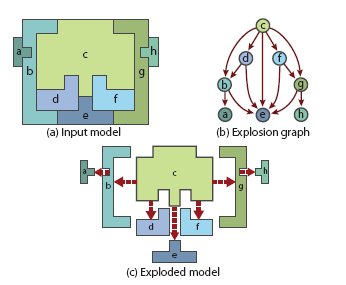
\includegraphics[height=125.0px]{img/exview3D-SIG08_2}
	\end{center}
\end{itemize}
\end{frame}

\begin{frame}\frametitle{\emph{Automated generation of interactive 3D exploded view diagrams} \cite{1360700}} 
\begin{itemize}
	\item Construindo o grafo explodido (\cite{882352}):
	\item S: conjunto com as partes ativas do modelo (ou seja, ainda n�o inseridas no grafo).
	\item P: sub-conjunto de S de partes que n�o possuam restri��o em pelo menos uma dire��o.
	\begin{enumerate}
		\item Determina P.
		\item Para cada parte $\emph{p} \in P$: determina a dist�ncia m�nima que \emph{p} teria que mover para sair do \emph{bounding box} das partes em contato com \emph{p}.
		\item \emph{p} com a menor dist�ncia � adicionado ao grafo. Arestas s�o adicionadas ligando \emph{p} a todas as outras partes que est�o em contato.
	\end{enumerate}
\end{itemize}
\end{frame}
\section{Proposta}

\begin{frame}\frametitle{Proposta} 
\begin{itemize}
	\item 
\end{itemize}	
\end{frame}

\section{Bibliografia}
\begin{tiny}
%\nocite{*}
\bibliographystyle{apalike}
\bibliography{INF2062_partial}
\end{tiny}



\end{document}
